\newpage
\section{Branch PC Generator}
The \texttt{branchPCGenerator} module is a crucial component in the control unit of a processor, implemented using Verilog, a hardware description language. This module determines the next value of the program counter (PC), which is essential for guiding the processor's instruction flow. It takes several inputs, including control signals and current state values, to decide whether to branch to a new address or continue sequentially. The primary inputs to this module are \texttt{branchControl}, \texttt{zeroFlag}, \texttt{newPC}, \texttt{curretPC}, and \texttt{immidiateValue}, while the output is the \texttt{nextPC}.

\begin{figure}[H]
    \centering
    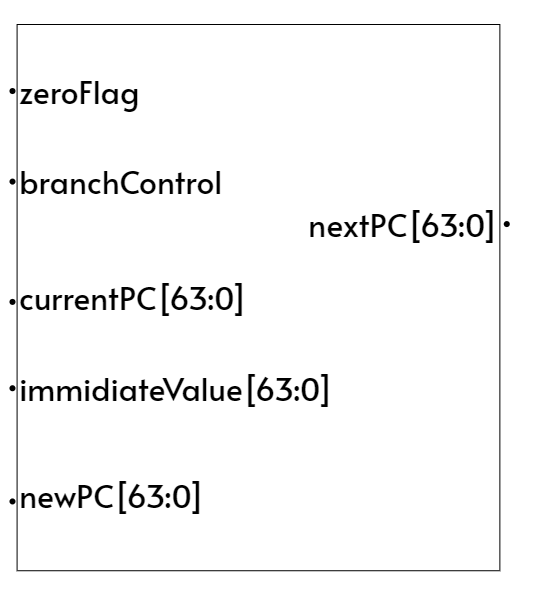
\includegraphics[width=0.3\textwidth, height=0.23\textheight]{Image/02_BPC.png}
    \caption{Branch PC generator}
    \label{fig:Branch PC generator}
\end{figure}

The inputs \texttt{branchControl} and \texttt{zeroFlag} are critical for branch decision-making. \texttt{branchControl} indicates whether a branch instruction is active, and \texttt{zeroFlag} reflects the outcome of a condition check, typically whether a computed result is zero. These signals are combined using a logical AND operation to produce the \texttt{branchDecision} signal. This signal is high only when both the branch control is asserted and the zero flag condition is met, indicating that a branch should be taken. 
\\ 
\hfill \break
The \texttt{nextPC} value is calculated based on the \texttt{branchDecision} signal. If \texttt{branchDecision} is high, indicating that a branch should be taken, \texttt{nextPC} is set to the current PC (\texttt{curretPC}) plus an immediate value (\texttt{immidiateValue}) shifted left by one bit. The left shift operation effectively multiplies the immediate value by two, a common technique used in instruction set architectures for byte addressing with word-aligned instructions. This operation ensures that the processor can jump to the correct instruction address specified by the branch. 
\\ 
\hfill \break
If \texttt{branchDecision} is low, indicating that the branch condition is not met, the \texttt{nextPC} is set to \texttt{newPC}, which represents the next sequential instruction address. This conditional assignment, resembling a multiplexer function, ensures that the processor continues to execute instructions in the correct order, either by branching to a new address or moving to the next sequential address. Thus, the \texttt{branchPCGenerator} module enables efficient control flow management within the processor, ensuring that branch instructions are correctly handled based on the given conditions.


